\documentclass{article}

\usepackage[utf8]{inputenc}
\usepackage[T1]{fontenc}      
\usepackage[francais]{babel}
\usepackage{chemist}
\usepackage{chemfig} 
\usepackage{lewis}
\usepackage[top=2.5cm,bottom=2.5cm,right=2.5cm,left=2.5cm]{geometry}
\usepackage[squaren, Gray]{SIunits}
\usepackage{url}
\usepackage{hyperref}
\usepackage[numbered, framed]{mcode}
\hypersetup{
    colorlinks,
    citecolor=black,
    filecolor=black,
    linkcolor=black,
    urlcolor=black
}

\newcommand\chemfigc[1]{
\vspace{0.5cm}
\begin{center}\chemfig{#1}\end{center}
\vspace{0.5cm}}

\title{Projet 3 - Rapport de tâche 1}
\author{\textbf{Groupe 124.3}
\\
\textsc{Frenyo} P\'eter (6266-12-00)\\
\textsc{Gillain} Nathan (7879-12-00)\\
\textsc{Lamine} Guillaume (7109-13-00)\\
\textsc{Piraux} Pauline (2520-13-00)\\
\textsc{Paris} Antoine (3158-13-00)\\
\textsc{Quiriny} Simon (4235-13-00)\\
\textsc{Schrurs} Sébastien (7978-13-00)}
\date{\today} 
\begin{document}

\maketitle
\tableofcontents

\section{Calcul du flux des réactifs}

\paragraph{Hypothèse}
Lors du calcul de ces flux, nous avons utilisé l'hypothèse que tous les réactifs sont 
consommés par le réacteur.

\paragraph{Calculs}
L'équation de la réaction de production de l'ammoniac par le procédé \textsc{Haber-Bosch} est donnée par :

	\begin{chemmath}
			\frac{1}{2}N_2(g) + \frac{3}{2}H_2(g) \longrightarrow NH_3(g) + \Delta H
 	\end{chemmath}
	
En sachant que l'on cherche à produire \unit{1000}{\ton} de \chemform{NH_3} par jour, 
on calcule assez facilement le flux de \chemform{N_2} (les détails de calculs ont été omis
dans ce rapport)

	$$m_{N_2} = \unit{823.5}{\ton\per\dday}$$

et le flux de \chemform{H_2}

	$$m_{H_2} = \unit{176.4}{\ton\per\dday}.$$

\section{Calcul du débit d'eau nécessaire pour refroidir le réactif}
\paragraph{Hypothèses}
\begin{itemize}
	\item Les capacités calorifiques ne dépendent pas de la température ;
	\item La pression dans le réacteur est constante et vaut \unit{10^5}{\pascal}.
\end{itemize}

\paragraph{Première méthode : on considère les capacités calorifiques constantes}
Pour la réaction donnée dans la section précédente, on a $\Delta H(\unit{298.15}{\kelvin})
 = \unit{-46 \cdot 10^3}{\joule}$ pour une mole de \chemform{NH_3(g)} produite \cite{atkins}.
Comme la réaction a lieu à \unit{500}{\celsius} (c'est à dire \unit{773.15}{\kelvin}), il
va falloir calculer $\Delta H(\unit{773.15}{\kelvin})$. Pour cela, nous avons besoin
des capacités calorifiques moyenne à pression constante de chacun des réactifs et des produits
de la réaction. Nous trouvons ces données dans une table \cite{atkins}.

	$$
	\left\{
		\begin{array}{rl}
			C_{p_{NH_3(g)}} &= \unit{37}{\joule\per\mole\kelvin}\\
			C_{p_{H_2(g)}} 	&= \unit{28.836}{\joule\per\mole\kelvin}\\
			C_{p_{N_2(g)}} 	&= \unit{29.124}{\joule\per\mole\kelvin}
		\end{array}
	\right
	$$

On a donc :

$$\Delta H(\unit{773.15}{\kelvin}) = \Delta H(\unit{298.15}{\kelvin})
+ \int_{298.15}^{773.15} C_{p_{NH_3(g)}} dT - \frac{1}{2}\int_{298.15}^{773.15} C_{p_{N_2(g)}} dT
- \frac{3}{2} \int_{298.15}^{773.15} C_{p_{H_2(g)}} dT = \unit{-5.5887 \cdot 10^4}{\joule\per\mole}$$

Pour la quantité de \chemform{NH_3} à produire par jour (à savoir $\unit{58.83 \cdot 10^6}{\mole}$),
la quantité de chaleur produite est donc :

$$q = \Delta H(\unit{773.15}{\kelvin}) \cdot n_{NH_3} = \unit{-3.28786 \cdot 10^{12}}{\joule}$$

En connaissant la capacité calorifique de l'eau $C_{H_2O(g)} = \unit{4185.5}{\joule\per\kilo\gram\kelvin}$ \cite{atkins}et en égalant
$q$ à $m_{H_2O} \cdot C_{H_2O(g)} \cdot \Delta T$ avec $\Delta T = 90 - 25 = \unit{65}{\kelvin}$, on trouve un
flux d'eau égal à

$$m_{H_2O} = \unit{1.2085 \cdot 10^7}{\kilo\gram\per\dday} \Rightarrow V_{H_2O} \approx \unit{1.2085 \cdot 10^7}{\liter\per\dday} 
= \unit{139.8}{\liter\per\second}$$

\paragraph{Deuxième méthode : les capacités calorifiques dépendent de la température}
On peut être plus précis en utilisant les capacités calorifiques suivantes \cite{hc-table} :

	$$
	\left\{
		\begin{array}{rl}
			C_{p_{NH_3(g)}}(T) &= \unit{31.81 + (15.48 \cdot 10^{-3})T + (5.86 \cdot 10^{-6})T^2}{\joule\per\mole\kelvin}\\
			C_{p_{H_2(g)}}(T) 	&= \unit{29.30 - (0.84 \cdot 10^{-3})T + (2.09 \cdot 10^{-6})T^2}{\joule\per\mole\kelvin}\\
			C_{p_{N_2(g)}}(T) 	&= \unit{27.62 + (4.19 \cdot 10^{-3})T}{\joule\per\mole\kelvin}
		\end{array}
	\right
	$$

En refaisant le calcul ci-dessus en tenant compte de la variation des capacités calorifiques en fonction
de la température, nous obtenons un débit un peu inférieur de \unit{135.662}{\liter\per\second}. On remarque
que l'approximation faite ci-dessus n'est pas si mauvaise que ça. Nous vous épargons ici
les détails de calculs (que nous avons réalisé avec \textsc{Matlab}).

\section{Sources des réactifs}
	\subsection{Sources de diazote}
	\subsubsection{Procédé cryogénique}
	Ce procédé se base sur la séparation des différents constituants de l'air en fonction de leur température 
	d'ébullition (l'oxygène \chemform{O_2} se condense avant le diazote \chemform{N_2}).
	L'air est purifié jusqu'à liquéfaction et les différents constituants sont séparés dans une colonne de 
	rectification par distillation fractionnée. Cette méthode permet d'avoir du diazote \chemform{N_2} pur 
	à \numprint{99,99}\%. Cette méthode est efficace pour une consommation au-delà de $\unit{200}{\meter\cubed\per\hour}$ \cite{scf}. 

	\subsubsection{Perméation gazeuse}
	Ce procédé utilise les différentes vitesses d'effusion des molécules de gaz à travers une membrane. 
	L'\chemform{O_2}, \chemform{H_2O} et le \chemform{CO_2} s'effusent plus rapidement que le \chemform{N_2}.
	Cette méthode nous permet d'obtenir du \chemform{N_2} sec pur à \numprint{95-99}. Ce procédé s'utilise pour des 
	débits forts variables ($\unit{3-1000}{\meter\cubed\per\hour}$) \cite{scf}.

	\subsubsection{Méthode de Ramsay}
	
	\begin{chemmath}
			NaNO_2(aq) + NH_4Cl(aq) \longrightarrow NaCl(aq) + 2 H_2O(l) + N_2(g)
	\end{chemmath}
	
	On chauffe le mélange de \chemform{NaNO_2} et \chemform{NH_4Cl} pour obtenir le \chemform{N_2} sous forme gazeuse.
	Un désavantage de cette méthode par rapport aux 2 premières est qu'il faut acheter les réactifs. De plus, il faut utiliser de l'énergie pour chauffer la réaction \cite{wiki-n2}.

	\subsection{Sources de dihydrogène}
		\subsubsection{Vaporeformage de méthane}
		2 réactions sont utilisées pour ce procédé \cite{afhypac} :
		
		\begin{chemmath} 
			CH_4 + H_2O \longleftrightarrow CO + 3H_2
		\end{chemmath}
		
		\begin{chemmath}
			CO + H_2O \longleftrightarrow CO_2 + H_2
		\end{chemmath}
		
		L'équation bilan obtenue est la suivante :
		
		\begin{chemmath}
			CH_4 + 2H_2O \longleftrightarrow CO_2 + 4 H_2
		\end{chemmath}
		
			Cette réaction nécessite un catalyseur : le nickel. Le rendement varie entre $40-45\%$. Le problème de cette 
			méthode est qu'elle rejette une grande quantité de \chemform{CO_2}, gaz à effet de serre \cite{wiki-h2}.
			
		\subsubsection{Oxydation partielle d'hydrocarbure}
		\begin{chemmath}
			C_nH_m + \frac{n}{2} O_2 + \frac{3,76n}{2} N_2 \longrightarrow \frac{m}{2} H_2 + n CO + \frac{3,76n}{2} N_2
		\end{chemmath}
		L'air est comburant pour cette réaction, qui a besoin d'être catalysée. Son caractère exothermique aide à la catalyse. 
		L'inconvénient de cette méthode est son faible rendement \cite{wiki-h2}.

		\subsubsection{Electrolyse}
		Réaction à l'anode : 
		
		\begin{chemmath}
			2H_2O(l) \longrightarrow O_2(g) + 4 H^+(aq) + 4e^-
		\end{chemmath}
		
		Réaction à la cathode :
		
		\begin{chemmath}
			4H_2O(l) + 4e^- \longrightarrow 2H_2O(g) + 4OH^-(aq)
		\end{chemmath}
		
		L'équation bilan obtenue est la suivante :
		
		\begin{chemmath}
			2H_2O(l) \longrightarrow 2H_2(g) + O_2(g)
		\end{chemmath}
		
	La réaction nécessite une grande quantité d'électricité. L'eau, quant à elle, est présente en quantité illimitée 
	et est peu coûteuse. En pratique, cette méthode est très peu utilisée \cite{wiki-h2}.

\section{Bilan de matiere}
On pose le flux de \chemform{NH_3(g)} à la sortie égal à $\unit{m_{NH_3}}{\gram\per\dday}\footnote{Avec \unit{\gram\per\day} = grammes par jour.}$. 

Nous partons de la réaction : 
\begin{chemmath}
		\frac{1}{2}N_2(g) + \frac{3}{2}H_2(g) \longrightarrow NH_3(g) 
\end{chemmath}
 	
$$m_{NH_3} = \unit{m_{NH_3}}{\gram\per\dday}$$ 

Et donc, 
 
$$n_{NH_3} = \unit{\frac{m_{NH_3}}{17}}{\mole}$$

Ce qui donne 

$$n_{N_2} = \frac{n_{NH_3}}{2} = \unit{\frac{m_{NH_3}}{34}}{\mole}$$ 

et 

$$n_{H_2} = \frac{3}{2} \cdot n_{NH_3}$$

On sait que le \chemform{N_2(g)} provient uniquement de l'air entrant 
dans le réacteur du  réformage primaire. Et comme on poser comme hypothèse
que l'air est composé de 78\% de \chemform{N_2(g)}, 21\% de \chemform{O_2(g)}
et 1\% d'\chemform{Ar(g)}, on peut déduire que $n_{air}$ entrant dans le 
réacteur du réformage primaire vaut : 

$$n_{air}= n_{N_2} \cdot \frac{100}{78} = \unit{\frac{25m_{NH_3}}{663}}{\mole}$$ 

Et :
$$n_{O_2}= n_{air} \cdot \frac{21}{100} = \unit{\frac{7m_{NH_3}}{884}}{\mole}$$
$$n_{Ar}= n_{air} \cdot \frac{1}{100} = \unit{\frac{1m_{NH_3}}{2652}}{\mole}$$

On sait par la réaction du réformage primaire suivante:
\begin{chemmath}
	2CH_4 + O_2 \Longrightarrow 2CO + 4 H_2
\end{chemmath}  

et par l'hypothèse que le
\chemform{CH_4(g)} et le \chemform{O_2(g)} sont présents en quantité stoechiométrique : 

$$n_{CH_4} = 2 \cdot n_{O_2} = \unit{\frac{7m_{NH_3}}{442}}{\mole}$$
$$n_{CO} = n_{CH_4} =  \unit{\frac{7m_{NH_3}}{442}} {\mole}$$
$$n_{H_2} = 2 \cdot n_{CH_4} =  \unit{\frac{7m_{NH_3}}{221}}{\mole}$$

On s'intéresse ensuite à la réaction du Water-Gas-Shift : 

\begin{chemmath}
	CO + H_2O \Longrightarrow CO_2 + H_2
\end{chemmath} 

On sait que $n_{CO}-\text{WGS}$  = $n_{CO}-\text{réformage primaire}$ 
$+ n_{CO}\text{réformage secondaire}$ 

Et donc on a : 

$$n_{CO_2} = n_{CO} = n_{H_2O}$$

S'il reste du \chemform{H_2O} à la fin de cette réaction, $n_{H_2O}$ 
sera égal à $n_{H_2O}$ du réformage primaire moins le $n_{CO}$ du WGS.

On peut aussi déduire que $n_{CO_2-tot} = n_{{CO_2}-\text{réformage primaire}}
+ n_{{CO_2}-\text{WGS}}$.

On peut aussi conclure que : 

$$n_{H_2-\text{réformage primaire}}= n_{H_2-\text{synthèse \chemform{NH_3}}}
- n_{H_2-\text{réformarge secondaire}} - n_{H_2-\text{WGS}}$$

\section{Equilibre du reformage primaire}

\subsection{Calcul de la constante d'équilibre}

Pour calculer la constante d'équilibre nous allons utiliser $K= \exp{\frac{-\Delta G}{RT}}$ avec $\Delta G = \Delta H - T \Delta S $

\subsubsection{Première équation}
\begin{chemmath} 
 CH_4(g) + H_{2}O(g) \longrightarrow CO(g) + 3H_2
\end{chemmath} 

Connaissant l'enthalpie en conditions standards \cite{atkins} et les capacités calorifiques dépendant de la température \cite{hc-table}:
$$
\left\{
	\begin{array}{rl}
		C_{p_{CO}}(T) 			&= \unit{27.62 +(5.02 \cdot 10^{-3})T}{\joule\per\mole\kelvin} \\
		C_{p_{H_{2}}}(T) 		&= \unit{29.3-(0.84 \cdot 10^{-3})T + (2.09\cdot 10^{-6})T^2}{\joule\per\mole\kelvin} \\
		C_{p_{CH_{4}}}(T) 	&= \unit{14.23+(75.3 \cdot 10^{-3})T - (18\cdot 10^{-6})T^2}{\joule\per\mole\kelvin} \\
		C_{p_{H_{2}O}}(T) 	&= \unit{30.13+(10.46 \cdot 10^{-3})T}{\joule\per\mole\kelvin} 
	\end{array}
\right
$$

$$
	\begin{array}{rl}
		 	 \Delta H_1(T)	&=   \Delta H(\unit{298.15}{\kelvin}) 
												 + \int_{298.15}^{T} C_{p_{CO(g)}} dT + 3\int_{298.15}^{T} C_{p_{H_2(g)}} dT 
												 +  \int_{T}^{298.15} C_{p_{CH_4(g)}} dT + \int_{T}^{298.15}C_{p_{H_{2}O_{(g)}}}dT\\
											&= 188369.87 + 71.16 T -0.04163 T^2 + (8.09\cdot 10^{-6}) T^3 
	\end{array}
$$	

Connaisant l'entropie en conditions standards \cite{atkins}
 
$$
	\begin{array}{rl}
		 	 \Delta S_1(T)	&=  \Delta S(\unit{298.15}{\kelvin}) 
													 + \int_{298.15}^{T} C_{p_{CO(g)}} \frac{dT}{T} + 3\int_{298.15}^{T} C_{p_{H_2(g)}} \frac{dT}{T} 
													 +  \int_{T}^{298.15} C_{p_{CH_4(g)}} \frac{dT}{T} + \int_{T}^{298.15}C_{p_{H_{2}O_{(g)}}}\frac{dT}{T} \\
											&= -167.05 + 71.16 \ln T -0.08326 T + (1.2135\cdot 10^{-5}) T^2
	\end{array}
$$	

 Nous pouvons calculer $\Delta G_1$:
 
 $$
 \Delta G_1(T) = 188369.9 - (71.16\ln T)T + 238.21T + 0.04163 T^2 -(4.045\cdot 10^{-6})T^3
 $$ 

Nous obtenons donc
$$K_1 = \exp{\frac{-\Delta G_1}{RT}}$$
avec la valeur de $\Delta G_1$ calculée plus tôt.

\subsubsection{Deuxième équation}
\begin{chemmath} 
 CO(g) + H_{2}O(g) \longrightarrow CO_2(g) + H_2
\end{chemmath} 

Connaissant l'enthalpie en conditions standards \cite{atkins} et les capacités calorifiques dépendant de la température \cite{hc-table}:

$$
\begin{array}{rl}
C_{p_{CO_2}}(T)=32.22 +(22.18 \cdot 10^{-3})T + (3.35 \cdot 10^{-6})T^2\\
\end{array}
$$

$$
	\begin{array}{rl}
		 \Delta H_2(T)	&=  \Delta H(\unit{298.15}{\kelvin}) 
												 + \int_{298.15}^{T} C_{p_{CO_2(g)}} dT + \int_{298.15}^{T} C_{p_{H_2(g)}} dT 
												 +  \int_{T}^{298.15} C_{p_{CO(g)}} dT + \int_{T}^{298.15}C_{p_{H_{2}O_{(g)}}}dT \\
										&=  -42533.33+3.77T+(2.93\cdot 10^-3)T^2-(4.2\cdot 10^-7)T^3
	\end{array}
$$	

Connaisant l'entropie en conditions standards \cite{atkins}

$$
	\begin{array}{rl}
		 	\Delta S_2(T)	&=  \Delta S(\unit{298.15}{\kelvin}) 
											 + \int_{298.15}^{T} C_{p_{CO_2(g)}} \frac{dT}{T} + 3\int_{298.15}^{T} C_{p_{H_2(g)}} \frac{dT}{T} 
											 +  \int_{T}^{298.15} C_{p_{CO(g)}} \frac{dT}{T} + \int_{T}^{298.15}C_{p_{H_{2}O_{(g)}}}\frac{dT}{T}\\
										&=   -65.9 + 3.77 \ln(T) +(5.86\cdot 10^{-3})T -(6.3 \cdot 10^{-7})T^2
	\end{array}
$$	

Nous pouvons calculer $\Delta G_2$:
 
 $$
 \Delta G_2=-42533.33 - (3.77 \ln(T))T +69.67 T -(2.93 \cdot 10^{-3})T^2
 + (2.1\cdot 10^{-7})T^3 
 $$
 
Nous obtenons donc
$$K_2 = \exp{\frac{-\Delta G_2}{RT}}$$
avec la valeur de $\Delta G_2$ calculée plus tôt.

\subsection{Etat d'avancement}
Analysons maintenant plus en détails les deux réactions qui ont lieu dans le réformage primaire.
Ces deux réactions se passent à l'équilibre dans le même réacteur. 
De plus, dans la gamme de températures qui nous intéressent, on considère tous les composantes à l'état gazeux.
Nous ferons l'hypothèse que ces gazs se comportent comme des gazs parfaits.
Voici donc les tableaux d'avancement en conséquence, à la figure \ref{avancement}.
  
	\begin{figure}[htb!]
		\centering
		\includegraphics[scale=1.0]{avancements.png}
		\caption{Les tableaux d'avancement des deux réactions;}
		\label{avancement}
	\end{figure}
  
Ici, $x$ et $y$ sont respectivement les avancements des première et deuxième réactions. Nous travaillons en moles.
On remarque bien que les quantités à l'équilibre correspondent dans les deux tableaux.
Avant de s'attaquer à l'écriture des quotients réactionnels à l'équilibre, notons que le nombre total de moles de gaz
se trouve en prenant une seule fois le nombre de moles de chaque composant.
    
On a donc : $n_{g,tot} = n_{01} + n_{02} + 2x$ 
  
Nous pouvons écrire nos deux équilibres : 
 
$$
	\left\{
		\begin{array}{rl}
			K_1 =& \frac{(x-y)(3x+y)^3p_tot^2}{(n_{02}-x)(n_{02}-x-y)n_{g,tot}p_0^2} \\
			K_2 =& \frac{y(3x+y)}{(x-y)(n_{02-x-y})}
		\end{array}
	\right
$$

Pour ces équations, $p_{tot}$ est la pression à la sortie du réacteur, c'est-à-dire 28 bars
et $p_0$ est la pression standard, c'est à dire 1 bar.
$K_1$ et $K_2$ ont été calculés plus tôt en fonction de la température. 
De plus, grâce au bilan de matière fait précédement, nous obtenons les deux équations suivantes :

$$
	\left\{
		\begin{array}{rl}
			n_{01} - x =& \frac{7}{442} \cdot m_{NH_3} \\
			3x + y		 =& \frac{9}{221} \cdot m_{NH_3} - (x-y)
		\end{array}
	\right
$$
 
Ainsi, nous avons un système de quatre équations à quatre inconnues qui nous permettra d'exprimer
toutes les entrées/sorties en fonction de la température et de la masse de \chemform{NH_3}. 
   
\section{Bilan d'energie}
Afin d'évaluer la quantité totale d'énergie dont nous avons besoin pour mener à 
bien la synthèse d'ammoniac, nous allons regarder les quantités requises à chaque 
étape du processus pour ensuite déterminer la totalité des besoins énergétiques du
systéme.

Comme chaque réaction se passe à des températures différentes de la température ambiante,
nous calculerons le $\Delta H_{reaction}$ à température ambiante selon l'équation suivante 
$$\Delta H_{reaction} = \Sigma \Delta H_{f,produits} - \Sigma \Delta H_{f,reactifs}$$.

Ensuite, à l'aide des $C_{p}$ variables en fonction de la température, nous serons alors en 
mesure de déterminer le $\Delta H_{reaction}$ à la température voulue selon l'équation

$$\Delta H(T_2) = \Delta H(T_{1}) 
+ \int_{T_2}^{T_1} C_{p_{reactifs}} dT + \int_{T_1}^{T_2} C_{p_{produits}} dT$$ 

où $T_1$ est ici la température ambiante, soit \unit{298.15}{\kelvin}.

\paragraph{\'Equation de combustion}
La combustion du méthane se passe dans le four, et fournit la totalité de l'énergie 
requise par l'ensemble du processus, avec un rendement de 75 pourcents.
La réaction se produit selon l'équation chimique suivante :

\begin{chemmath}
	CH_4 + 2O_2 \Longrightarrow CO_2 + 4 H_2O
\end{chemmath}

$$
	\begin{array}{rl}
	\Delta H_{reaction}		&=  \Sigma \Delta H_{f,produits} - \Sigma \Delta H_{f,reactifs} \\
												&=  (-393.51) + 2\cdot(-241.82) - (-74.81) + 2\cdot0 \\
												&=  (-877.15) - (-74.81)\\
												&=  \unit{-802.34}{\kilo\joule\per\mole}
	\end{array}
$$

La réaction se passe généralement à une température avoisinant les $\unit{1300}{\kelvin}$.
Voici les $C_p$ variables en fonction de la température des différents composants\cite{hc-table} 
(exprimés en \unit{\joule\per\mole\kelvin}) :

$$
	\left\{
		\begin{array}{rl}
			C_{p_{CH_4}}(T) 	&= 14.23 + 75.3\cdot10^{-3}T + (-18\cdot10^{-6})T^2 \\
			C_{p_{O_2}}(T) 		&= 25.73 + 12.97\cdot10^{-3}T + (-3.77\cdot10^{-6})T^2 \\
			C_{p_{CO_2}}}(T) 	&= 32.22 + 22.18\cdot10^{-3}T + (-3.35\cdot10^{-6})T^2 \\
			C_{p_{H_2O}}(T) 	&= 30.13 + 10.46\cdot10^{-3}T + (0\cdot10^{-6})T^2 
		\end{array}
	\right
$$	

Calculons maintenant le $\Delta H$ pour une température $T_2$ de $\unit{1300}{\kelvin}$ :

$$
	\begin{array}{rl}
		 	\Delta H(\unit{1300}{\kelvin}) 	&=  \Delta H(\unit{298.15}{\kelvin}) + \int_{1300}^{298.15} C_{p_{reactifs}} dT + \int_{298.15}^{1300} C_{p_{produits}} dT \\
																			&=  \unit{-805.99}{\kilo\joule}
	\end{array}
$$	

On peut donc voir que cette réaction est largement exothermique, c'est elle qui fournira l'énergie nécessaire aux réactions du réformage primaire.

% J'ai retiré cette partie, personne ne la lire jamais.
%$ \\= \Delta H(\unit{298.15}{\kelvin}) + \int_{1300}^{298.15} C_{p_{CH_{4}}} dT +2\int_{1300}^{298.15} C_{p_{O_{2}}} dT + \int_{298.15}^{1300} C_{p_{CO_{2}}} dT + 2\int_{1300}^{298.15} C_{p_{H_{2}O}} dT$
%$ \\= -802.34 kJ/mol 
%+\int_{1300}^{298.15} (14.23 + 75.3\cdot10^{-3}T + (-18\cdot10^{-6})T^2) dT 
%+2\int_{1300}^{298.15} (25.73 + 12.97\cdot10^{-3}T + (-3.77\cdot10^{-6})T^2) dT
%+\int_{298.15}^{1300} (32.22 + 22.18\cdot10^{-3}T + (-3.35\cdot10^{-6})T^2) dT 
%+2\int_{298.15}^{1300} (30.13 + 10.46\cdot10^{-3}T + (0\cdot10^{-6})T^2) dT$			
%$ \\= -802.34 kJ/mol 
%- [14.23T + \frac{75.3\cdot10^{-3}}{2}T^2 + (\frac{-18\cdot10^{-6}}{3})T^3]_{298.15}^{1300} 
%-2 [25.73T + \frac{12.97\cdot10^{-3}}{2}T^2 + (\frac{-3.77\cdot10^{-6}}{3})T^3]_{298.15}^{1300} 
%+ [32.22T + \frac{22.18\cdot10^{-3}}{2}T^2 + \frac{(-3.35\cdot10^{-6})}{3}T^3]_{298.15}^{1300}  
%+2 [30.13T + \frac{(10.46)\cdot10^{-3}}{2}T^2 + \frac{(0\cdot10^{-6})}{3}T^3]_{298.15}^{1300} $
%$ \\= -802340
%-(68945.5-7430.5)-2(41647.8-8214.57)+(58174.8-10562.6)+2(48007.7-9448.17)$		
%$ \\= -802340 - 61515 - 66866.46 + 47612.2 + 77119.06 $
%$ \\=  $

\paragraph{Reformage primaire}
Dans notre travail, la température du réformage primaire est un paramètre. Nous obtiendrons donc une enthalpie 
dépendant de la température. 
Le réformage primaire est composé de deux équations.

\subparagraphe{Première équation}
\begin{chemmath} 
 CH_4(g) + H_{2}O(g) \longrightarrow CO(g) + 3H_2
\end{chemmath} 

Connaissant l'enthalpie en conditions standards \cite{atkins} et les capacités calorifiques dépendant de la température \cite{hc-table}:
$$
\left\{
	\begin{array}{rl}
		C_{p_{CO}}(T) 			&= \unit{27.62 +(5.02 \cdot 10^{-3})T}{\joule\per\mole\kelvin} \\
		C_{p_{H_{2}}}(T) 		&= \unit{29.3-(0.84 \cdot 10^{-3})T + (2.09\cdot 10^{-6})T^2}{\joule\per\mole\kelvin} \\
		C_{p_{CH_{4}}}(T) 	&= \unit{14.23+(75.3 \cdot 10^{-3})T - (18\cdot 10^{-6})T^2}{\joule\per\mole\kelvin} \\
		C_{p_{H_{2}O}}(T) 	&= \unit{30.13+(10.46 \cdot 10^{-3})T}{\joule\per\mole\kelvin} 
	\end{array}
\right
$$

$$
	\begin{array}{rl}
		 	\Delta H_1(T) = \Delta H(\unit{298.15}{\kelvin})	&=  + \int_{298.15}^{T} C_{p_{CO(g)}} dT + 3\int_{298.15}^{T} C_{p_{H_2(g)}} dT 
																														+  \int_{T}^{298.15} C_{p_{CH_4(g)}} dT + \int_{T}^{298.15}C_{p_{H_{2}O_{(g)}}}dT\\
																												&=  188369.87 + 71.16 T -0.04163 T^2 + (8.09\cdot 10^{-6}) T^3
	\end{array}
$$	

\subparagraphe{Deuxième équation}
\begin{chemmath} 
 CO(g) + H_{2}O(g) \longrightarrow CO_2(g) + H_2
\end{chemmath} 

Connaissant l'enthalpie en conditions standards \cite{atkins} et les capacités calorifiques dépendant de la température \cite{hc-table}:

$$
\begin{array}{rl}
C_{p_{CO_2}}(T)=32.22 +(22.18 \cdot 10^{-3})T + (3.35 \cdot 10^{-6})T^2\\
\end{array}
$$

$$
	\begin{array}{rl}
		  \Delta H_2(T)	&=   \Delta H(\unit{298.15}{\kelvin}) 
											 + \int_{298.15}^{T} C_{p_{CO_2(g)}} dT + \int_{298.15}^{T} C_{p_{H_2(g)}} dT 
											 +  \int_{T}^{298.15} C_{p_{CO(g)}} dT + \int_{T}^{298.15}C_{p_{H_{2}O_{(g)}}}dT \\
										&=  -42533.33+3.77T+(2.93\cdot 10^-3)T^2-(4.2\cdot 10^-7)T^3
	\end{array}
$$	

%\begin{chemmath}
%		CH_4 + 2H_2O \Longleftrightarrow 4H_2 + CO_2
%	\end{chemmath}
%
%$$
%	\begin{array}{rl}
%	\Delta H_{reaction}		&= \Sigma \Delta H_{f,produits} - \Sigma \Delta H_{f,reactifs}\\
%												&= 4 \cdot 0 + -393.51 - (-74.81 + 2\cdot(-241.82))\\
%												&= -393.51 - (-558.45) \\
%												&= \unit{164.94}{\kilo\joule\per\mole}
%	\end{array}
% $$
%Pauline : SIMON tu dois mettre ici ton calcul du DeltaH en fonction de T !!!! à remplacer par toute cette merde , qui sert à rien, 

%On peut remarquer que cette réaction est endothermique et a besoin de l'énergie de la réaction de combustion pour pouvoir se réaliser.
% Simon: on n'observe plus vraiment ici car pas de valeur.
\paragraph{Reformage secondaire}

\begin{chemmath}
		CH_4 + \frac{1}{2}O_2 \Longrightarrow CO + 2H_2
\end{chemmath}

$$
	\begin{array}{rl}
	\Delta H_{reaction}		&= \Sigma \Delta H_{f,produits} - \Sigma \Delta H_{f,reactifs}\\
												&= (-110.53) + 2\cdot 0 - ((-74.81) + \frac{1}{2}\cdot 0)\\
												&=  (-110.53) - (-74.81)\\
												&=  -\unit{35.72}{\kilo\joule\per\mole}
	\end{array}
$$

Le reformage secondaire s'opere generalement a une temperature de $\unit{1173}{\kelvin}$.
Voici les $C_p$ variables en fonction de la température des différents composants\cite{hc-table} 
(exprimées en \unit{\joule\per\mole\kelvin}) :

$$
	\left\{
		\begin{array}{rl}
			C_{p_{CH_4}}(T) 	&= 14.23 + 75.3\cdot10^{-3}T + (-18\cdot10^{-6})T^2 \\
			C_{p_{O_2}}(T) 		&= 25.73 + 12.97\cdot10^{-3}T + (-3.77\cdot10^{-6})T^2 \\
			C_{p_{CO}}(T) 		&= 27.62 + 5.02\cdot10^{-3}T + (0\cdot10^{-6})T^2 \\
			C_{p_{H_2}}(T) 		&= 29.3 + (-0.84)\cdot10^{-3}T + (2.09\cdot10^{-6})T^2
		\end{array}
	\right
$$

Calculons maintenant le $\Delta H$ a $\unit{1173.15}{\kelvin}$ :

$$
	\begin{array}{rl}
		 	\Delta H(\unit{1173.15}{\kelvin}) &=  \Delta H(\unit{298.15}{\kelvin}) 
																						+ \int_{1173.15}^{298.15} C_{p_{reactifs}} dT + \int_{298.15}^{1173.15} 
																						C_{p_{produits}} dT \\
																				&=  \unit{-20.29}{\kilo\joule}
	\end{array}
$$	

Il s'agit donc d'une réaction exothermique.

% De nouveau, je retire les calculs un peu long.
%$ \\= \Delta H(\unit{298.15}{\kelvin}) + \int_{1173.15}^{298.15} C_{p_{CH_{4}}} dT +\frac{1}{2}\int_{1173.15}^{298.15} C_{p_{O_{2}}} dT + \int_{298.15}^{1173.15} C_{p_{CO}} dT + 2\int_{1173.15}^{298.15} C_{p_{H_{2}}} dT$
%$ \\= -35.72 kJ/mol 
%+\int_{1173.15}^{298.15} (14.23 + 75.3*10^{-3}T + (-18*10^{-6})T^2) dT 
%+\frac{1}{2}\int_{1173.15}^{298.15} (25.73 + 12.97*10^{-3}T + (-3.77*10^{-6})T^2) dT
%+\int_{298.15}^{1173.15} (27.62 + 5.02*10^{-3}T + (0*10^{-6})T^2) dT 
%+2\int_{298.15}^{1173.15} (29.3 + (-0.84)*10^{-3}T + (2.09*10^{-6})T^2) dT$			
%$ \\= -35.72 kJ/mol 
%- [14.23T + \frac{75.3*10^{-3}}{2}T^2 + (\frac{-18*10^{-6}}{3})T^3]_{298.15}^{1173.15} 
%-\frac{1}{2} [25.73T + \frac{12.97*10^{-3}}{2}T^2 + (\frac{-3.77*10^{-6}}{3})T^3]_{298.15}^{1173.15} 
%+ [27.62T + \frac{5.02*10^{-3}}{2}T^2 + \frac{(0*10^{-6})}{3}T^3]_{298.15}^{1173.15}  
%+2 [29.3T + \frac{(-0.84)*10^{-3}}{2}T^2 + \frac{(2.09*10^{-6})}{3}T^3]_{298.15}^{1173.15} $
%$ \\= -35720
%-(58823.4-7430.5) -\frac{1}{2}(37081-8214.57)+(35856.9-8458.03)+2(34920.1-7986.16)$		
%$ \\= -35720 - 51392.9 - 14433.215 + 27398.87 + 53867.88 $
%$ \\= -20.28 kJ $

\paragraph{Water-Gas-Shift}

\begin{chemmath}
		CO + H_2O \Longrightarrow H_2 + CO_2
\end{chemmath}	

$$
	\begin{array}{rl}
	\Delta H_{reaction}		&= \Sigma \Delta H_{f,produits} - \Sigma \Delta H_{f,reactifs} \\
												&= 0 + (-393.51) - (-110.53 + (-241.82)) \\
												&= -393.51 - (-352.35) \\
												&= \unit{-41.16}{\kilo\joule\per\mole}
	\end{array}
$$

Le Water Gas Shift s'opere generalement entre 200 et \unit{400}{\degree}. Nous considérerons
alors une température de réaction de $\unit{300}{\degree}$, soit $\unit{573.15}{\kelvin}$.
						
Voici les $C_{p}$ variables en fonction de la température des différents composants\cite{hc-table} :

$$
	\left\{
		\begin{array}{rl}
			C_{p_{CO_{2}}}(T) &= 32.22 + 22.18\cdot10^{-3}T + (-3.35\cdot10^{-6})T^2\\
			C_{p_{H_2O}}(T)		&= 30.13 + 10.46\cdot10^{-3}T + (0\cdot10^{-6})T^2\\
			C_{p_{CO}}(T) 		&= 27.62 + 5.02\cdot10^{-3}T + (0\cdot10^{-6})T^2 \\
			C_{p_{H_2}}(T) 		&= 29.3 + (-0.84)\cdot10^{-3}T + (2.09\cdot10^{-6})T^2
		\end{array}
	\right
$$
					
Calculons maintenant le $\Delta H$ à $\unit{573.15}{\kelvin}$ :			

$$
	\begin{array}{rl}
		 	 \Delta H(\unit{573.15}{\kelvin})	&=  \Delta H(\unit{298.15}{\kelvin}) 
																							+ \int_{573.15}^{298.15} C_{p_{reactifs}} dT + \int_{298.15}^{573.15} C_{p_{produits}} dT \\
																				&=  \unit{-55.63}{\kilo\joule}
	\end{array}
$$	
	
Il s'agit donc d'une réaction exothermique.

% Viré aussi
%$ \\= \Delta H(\unit{298.15}{\kelvin}) + \int_{573.15}^{298.15} C_{p_{CO}} dT +\int_{573.15}^{298.15} C_{p_{H_{2}O}} dT + \int_{298.15}^{573.15} C_{p_{CO_{2}}} dT + \int_{298.15}^{573.15} C_{p_{H_{2}}} dT$
%$ \\= -41.16 kJ/mol 
%+\int_{573.15}^{298.15} (27.62 + 5.04*10^{-3}T + (0*10^{-6})T^2) dT 
%+\int_{573.15}^{298.15} (30.13 + 10.46*10^{-3}T + (0*10^{-6})T^2) dT
%+\int_{298.15}^{573.15} (32.22 + 22.18*10^{-3}T + (-3.35*10^{-6})T^2) dT 
%+\int_{298.15}^{573.15} (29.3 + (-0.84)*10^{-3}T + (2.09*10^{-6})T^2) dT$			
%$ \\= -41.16 kJ/mol 
%- [27.62T + \frac{5.04*10^{-3}}{2}T^2 + (\frac{0*10^{-6}}{3})T^3]_{298.15}^{573.15} 
%- [30.13T + \frac{10.46*10^{-3}}{2}T^2 + (\frac{0*10^{-6}}{3})T^3]_{298.15}^{573.15} 
%+ [32.22T + \frac{22.18*10^{-3}}{2}T^2 + \frac{(-3.35*10^{-6})}{3}T^3]_{298.15}^{573.15}  
%+ [29.3T + \frac{(-0.84)*10^{-3}}{2}T^2 + \frac{(2.09*10^{-6})}{3}T^3]_{298.15}^{573.15} $
%$ \\= -41160
%-(16658.2-8458.91)-(18987.1-9448.17)+(21899.7-10562.6)+(16786.5-8716.92)$		
%$ \\= -41160 - 8199.29 - 9538.93 + 11337.1 + 8069.58 $
%$ \\= -55.63 kJ $

\paragraph{S\'eparation de $CO_{2}$ et de $H_{2}O$}		

Pour cette \'etape, nous ferons l'hypoth\`{e}se que les \'etapes requises pour enlever le $CO_{2}$ et le $H_{2}O$ des composants pr\'esents dans le circuit ne n\'ecessitent pas d'\'energie, ou du moins \'energ\'etiquement ind\'ependante des autres besoins en \'energie du reste du syst\`{e}me.

\paragraph{Synth\`{e}se du $NH_{3}$}		



\paragraph{Conclusion}
\'Etant donn\'e le fait que nous ayions besoin de X kiloJoules pour le reformage primaire, et que l'\'energie que la combustion donne au d\'ebut du syst\`{e}me se fait \`{a} un rendement de 75 pourcent, nous pouvons facilement d\'eterminer le d\'ebit de $CH_4$ \`{a} injecter dans le four au d\'epart. Cependant, la quantit\'e d'\'energie n\'ecessaire lors du reformage primaire varie en fonction de la temp\'erature. Par cons\'equent, la combustion sera aussi fonction de la temp\'erature, et ce en prenant en compte le rendement de 75 pourcent.
NB : "prendre en compte le rendement de 75 pourcent" signifie faire fonctionner le four \`{a} 133.3 pourcent afin d'avoir la quantit\'e d'\'energie n\'ecessaire malgr\'e le rendement inf\'erieur \`{a} 100 pourcent.


\section{Outil de gestion}
Notre outil de gestion se base sur les équations écrites lors du
bilan de matière et lors du calcul de l'état d'avancement des réactions
dans le reformage primaire. Il résout donc un système à 4 équations
et à 4 inconnues et ne sélectionne que les solutions positives. Notre programme
peut être amélioré et nous en sommes conscients. On pourrait le rendre plus robuste 
en traitant par exemple les cas ou les arguments de notre fonction ne sont pas 
valides. On peut aussi le rendre plus conviviale en créant un interface graphique
permettant d'utiliser notre fonction sans passer par la commande. On pourrait également
lui demander de calculer la quantité de \chemform{CO2} rejetée dans l'atmosphère afin
de quantifier l'impact environnemental. Toutes ces améliorations seront d'ailleurs ajoutées 
par la suite. Le code de notre fonction est présenté ci-dessous.

\lstinputlisting{OutilDeGestion.m}

\section{Calcul du nombre de tuyaux}
Maintenant, nous allons calculer le nombre de tubes dont nous aurons besoin pour
notre réacteur multi-tubulaire. Nous avons ces données de base : $\dot{m_{réactifs}} = \unit{517.05}{\ton\per\dday}$, 
$T = \unit{1080}{K}$, $d_{tube} = \unit{10^{-1}}{\meter}$ et $c = \unit{2}{\meter\per\second}$ où $\dot{m_{réactifs}}$ 
est le débit massique par jour de réactifs (déterminé avec l'outil de gestion pour une température citée ci-après et
un débit massique de $NH_{3}$ de $\unit{1500}{\ton\per\dday}$, $T$ une température plausible choisie pour le dimensionnement
du réacteur multi-tubulaire, $d_{tube}$ est le diamètre d'un tube et $c$ est la vitesse superficielle à l'entrée du réacteur.
Transformons d'abord le débit massique en débit volumique :

$$\unit{517.05}{\ton\per\dday} = \unit{5.984\cdot 10^{-3}}{\ton\per\second} = \unit{5.984\cdot \nu}{\meter^{3}\per\second} = \dot{V}$$

avec $\nu$ le volume massique du mélange que l'on introduit dans le réacteur. Nous pouvons déterminer $\nu$ grâce à 
l'expression de la loi des gaz parfaits sous forme thremodynamique $\nu = \frac{R^*\cdot T}{31\cdot 10^{5}}$ où $R^{*}$ vaut 

$$\frac{R}{\frac{16\cdot x_{CH_{4}}+18\cdot x_{H_{2}O}}{2}}}$$

avec $x_{CH_{4}$ et $x_{H_{2}O}$ les fractions molaire du méthane
et de l'eau entrant dans le système. Ensuite, à l'aide des notions de système ouvert et de l'hypothèse $\dot{m}_{\text{entrée}} = \dot{m}_{\text{sortie}}$,
nous obtenons que $\dot{V} = c \cdot  A$ avec $\dot{V}$ le débit volumique et $A$ la somme des sections de tous les tubes. 
En remplaçant par les valeurs que nous possédons, nous obtenons :

$$A = \frac{\dot{V}}{c} = \frac{5.984\dot \nu}{2} = \unit{2.992\cdot \nu}{\meter\squared}$$

Or, on sait que la surface d'un tube vaut $\pi\cdot (\frac{d}{2})^{2} = \unit{7.85\cdot 10^{-3}}{\meter\square}$. 
Le nombre de tubes est, dès lors, le rapport de la section totale trouvée plus haut sur la section d'un tube. 
Ce qui nous donne finalement : 

$$\text{Nombre de tubes} = \frac{2.992\cdot \nu}{7.854\cdot 10^{-3}} = 380.98\cdot \nu$$

Pour terminer cette partie, nous allons calculer un nombre de tuyaux sous certaines hypothèses et conditions.
Nous supposons que les fractions molaires de $CH_{4}$ et de $NH_{3}$ sont identiques (hypothèses valables à \unit{1080}{\kelvin}),
c'est-à-dire que $x_{CH_{4} = x_{H_{2}O}$. Dès lors, le volume massique $\nu$ devient:

$$\nu = \frac{R^{*}\cdot T}{31\cdot 10^{5}} = \frac{\frac{8.314}{17\cdot 10^{-3}}\cdot 1080}{31\cdot 10^{5}} = 0.17$$

Ce qui nous donne un nombre de tube approximatif de $65$ ($64.77$).

\bibliography{source-tache1}
\bibliographystyle{plain}
\nocite{*}

\appendix
\section{Annexes}
\subsection{Premier jet du flow-sheet simplifié}
La première ébauche de notre flow-sheet se trouve à la figure \ref{flow-sheet}.

\begin{figure}[htb!]
	\centering
	\rotatebox{90}{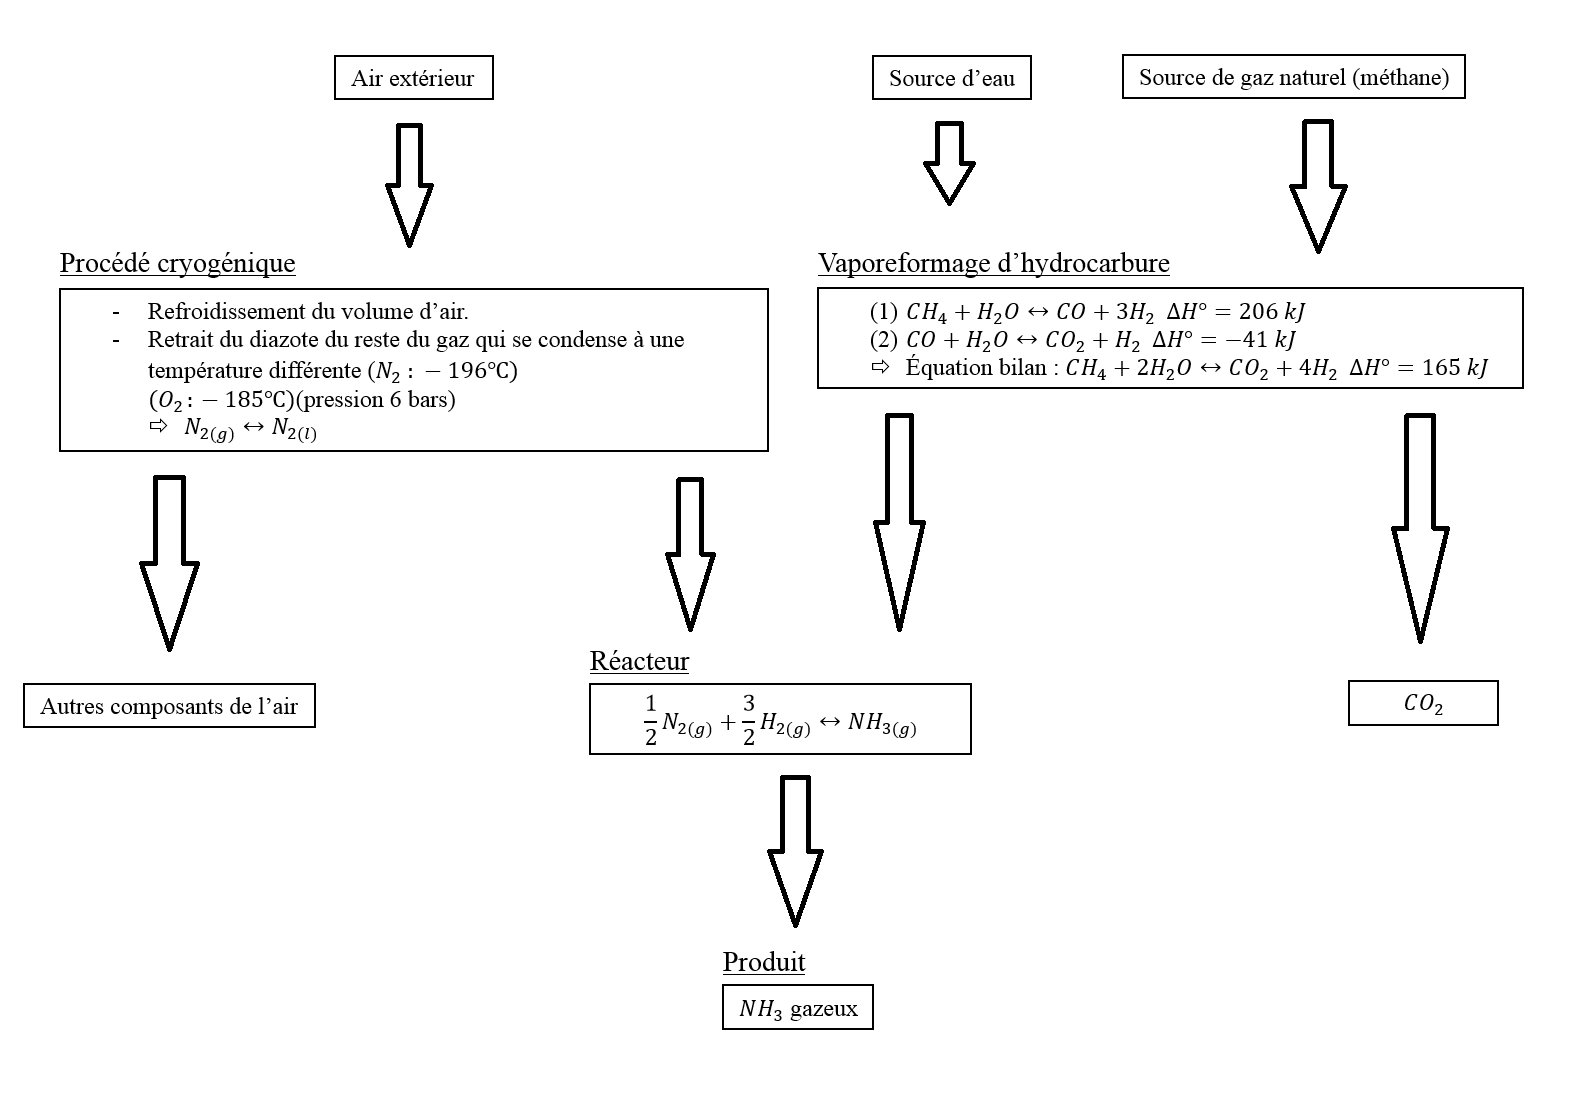
\includegraphics[scale=0.50]{flow-sheet.png}}
	\caption{Première ébauche de notre flow-sheet.}
	\label{flow-sheet}
\end{figure}

\subsection{Deuxième version du flow-sheet}
La deuxième version de notre flow-sheet se trouve à la figure \ref{flow-sheet-v2}.

\begin{figure}[htb!]
\centering
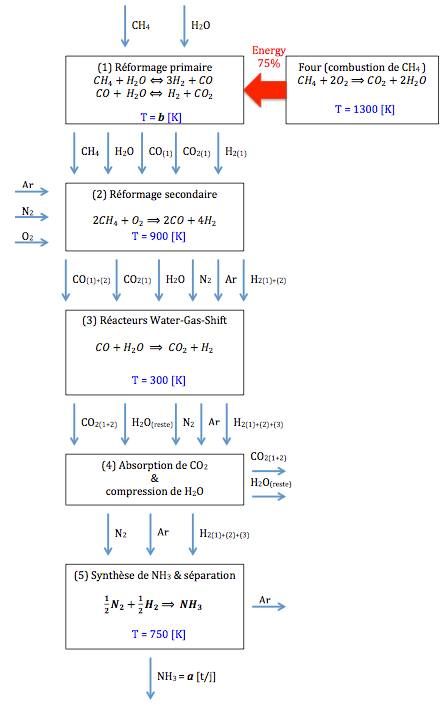
\includegraphics[scale=0.80]{flow-sheet-v2.jpg}
\caption{Deuxième ébauche de notre flow-sheet.}
\label{flow-sheet-v2}
\end{figure}

\end{document}
